
\chapter*{Introduzione}

Da qualche anno a questa parte sono stati sviluppati e messi in commercio dispositivi per la realtà virtuale, i più famosi sono la Nintendo Wii, il Kinect della Microsoft o l'Oculus Rift sviluppato da Oculus VR. Periferiche come queste sono chiamate NUI (natural user interface); esse  sono interfacce per l'interazione con sistemi virtuali, e hanno lo scopo di aumentare la sensazione della realtà durante l'utilizzo di applicazioni virtuali come i videogiochi, permettendo all'utente di sfruttare più sensi.

Il telecomando della Wii permette, indirettamente (dato il telecomando), di utilizzare il corpo umano come dispositivo di input di comandi. Il Kinect utilizza dei sensori a infrarossi e una telecamera per rilevare il corpo umano e registrare direttamente i suoi movimenti, trasformandoli in comandi di input. L'Oculus Rift è un visore che presenta dei sensori che riconoscono l'orientamento della testa, i cui movimenti sono tradotti in rotazioni della telecamera virtuale nell'applicazione, rendendo immersiva la visione, anche grazie alla presenza di due schermi che producono un effetto tridimensionale.

Il progetto trattato in questa tesi mira ad emulare dispositivi di questo genere, utilizzando semplicemente un computer e una webcam. Esso offre un'interfaccia che, tramite la webcam, utilizza la posizione del volto dell'utente per calcolare la prospettiva con cui viene visualizzata una scena tridimensionale, con lo scopo quindi di collegare la telecamera virtuale all'utente. L'obiettivo finale è quello di generare l'illusione della presenza di profondità all'interno dello schermo e di creare, quando le condizioni sono ottimali, un effetto tridimensionale senza l'utilizzo di occhiali appositi.

Dato l'utilizzo di software open source e di dispositivi di qualità media, l'effetto generato non è paragonabile a quello che può essere prodotto da sistemi più efficienti e dedicati allo scopo, tuttavia sono stati raggiunti comunque risultati notevoli.

I software impiegati nello sviluppo del progetto sono:
\begin{itemize}
\item OpenCv, per il rilevamento del volto.
\item OpenGl, per lo studio del metodo da utilizzare e per lo sviluppo dell'applicazione.
\item Blender, per la creazione di scene 3D.
\item Ogre3D, per un miglioramento dell'applicazione in termini di grafica ed efficienza.
\end{itemize}

Nel corso di questa tesi si introdurranno i software utilizzati, sarà spiegata la teoria matematica che sta dietro alle trasformazioni utilizzate, facendo un excursus sulle tecnice adottate dalla maggior parte delle applicazioni grafiche per renderizzare a chermo una scena tridimensionale, ed infine sarà trattato il progetto sviluppato, mostrando anche le problematiche riscontrate e le possibili soluzioni.Prima di tutto però, diamo dei brevi cenni riguardanti la realtà virtuale.

\begin{figure}[htbp]
\centering
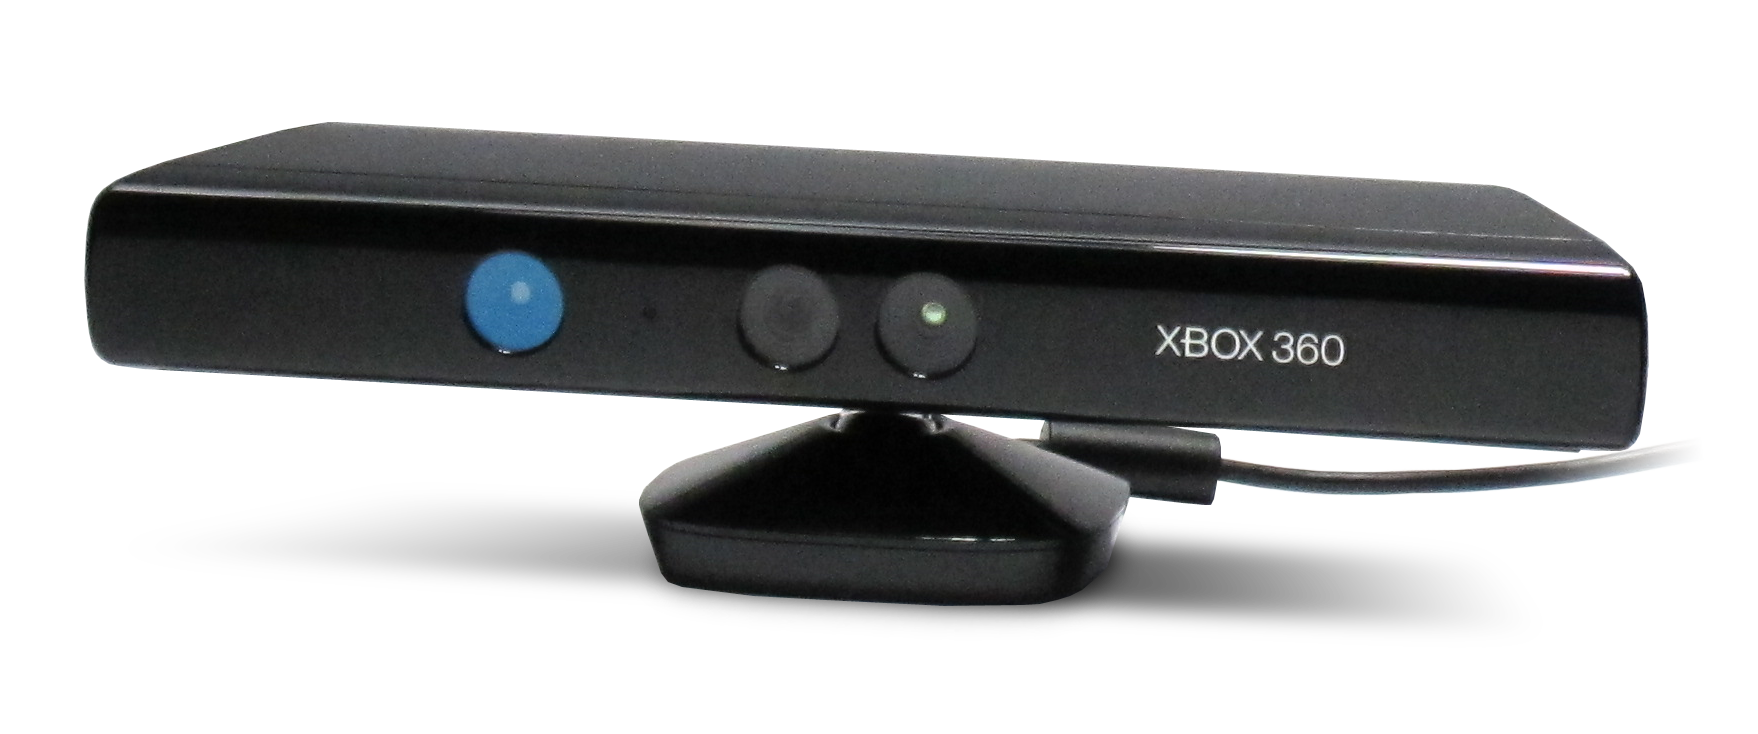
\includegraphics[width=0.4\textwidth]{images/intro/kinect.png}
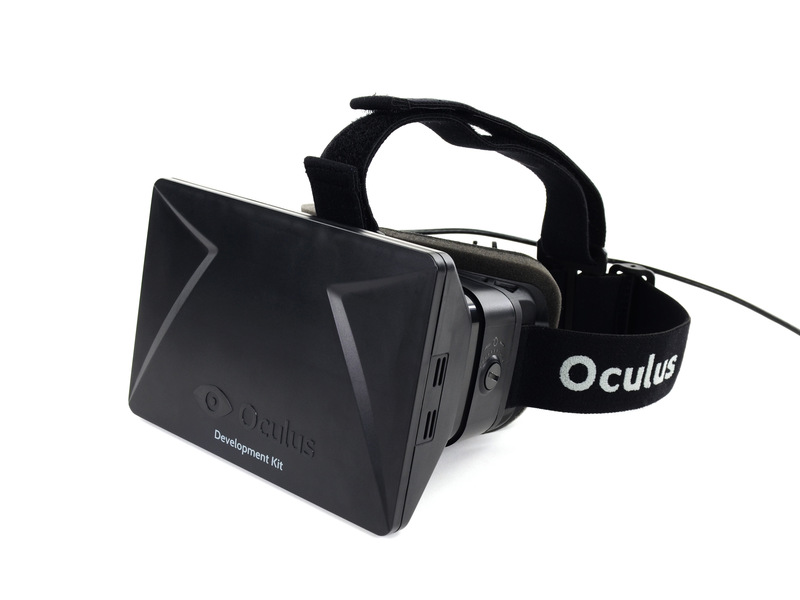
\includegraphics[width=0.4\textwidth]{images/intro/oculus-rift.jpg}
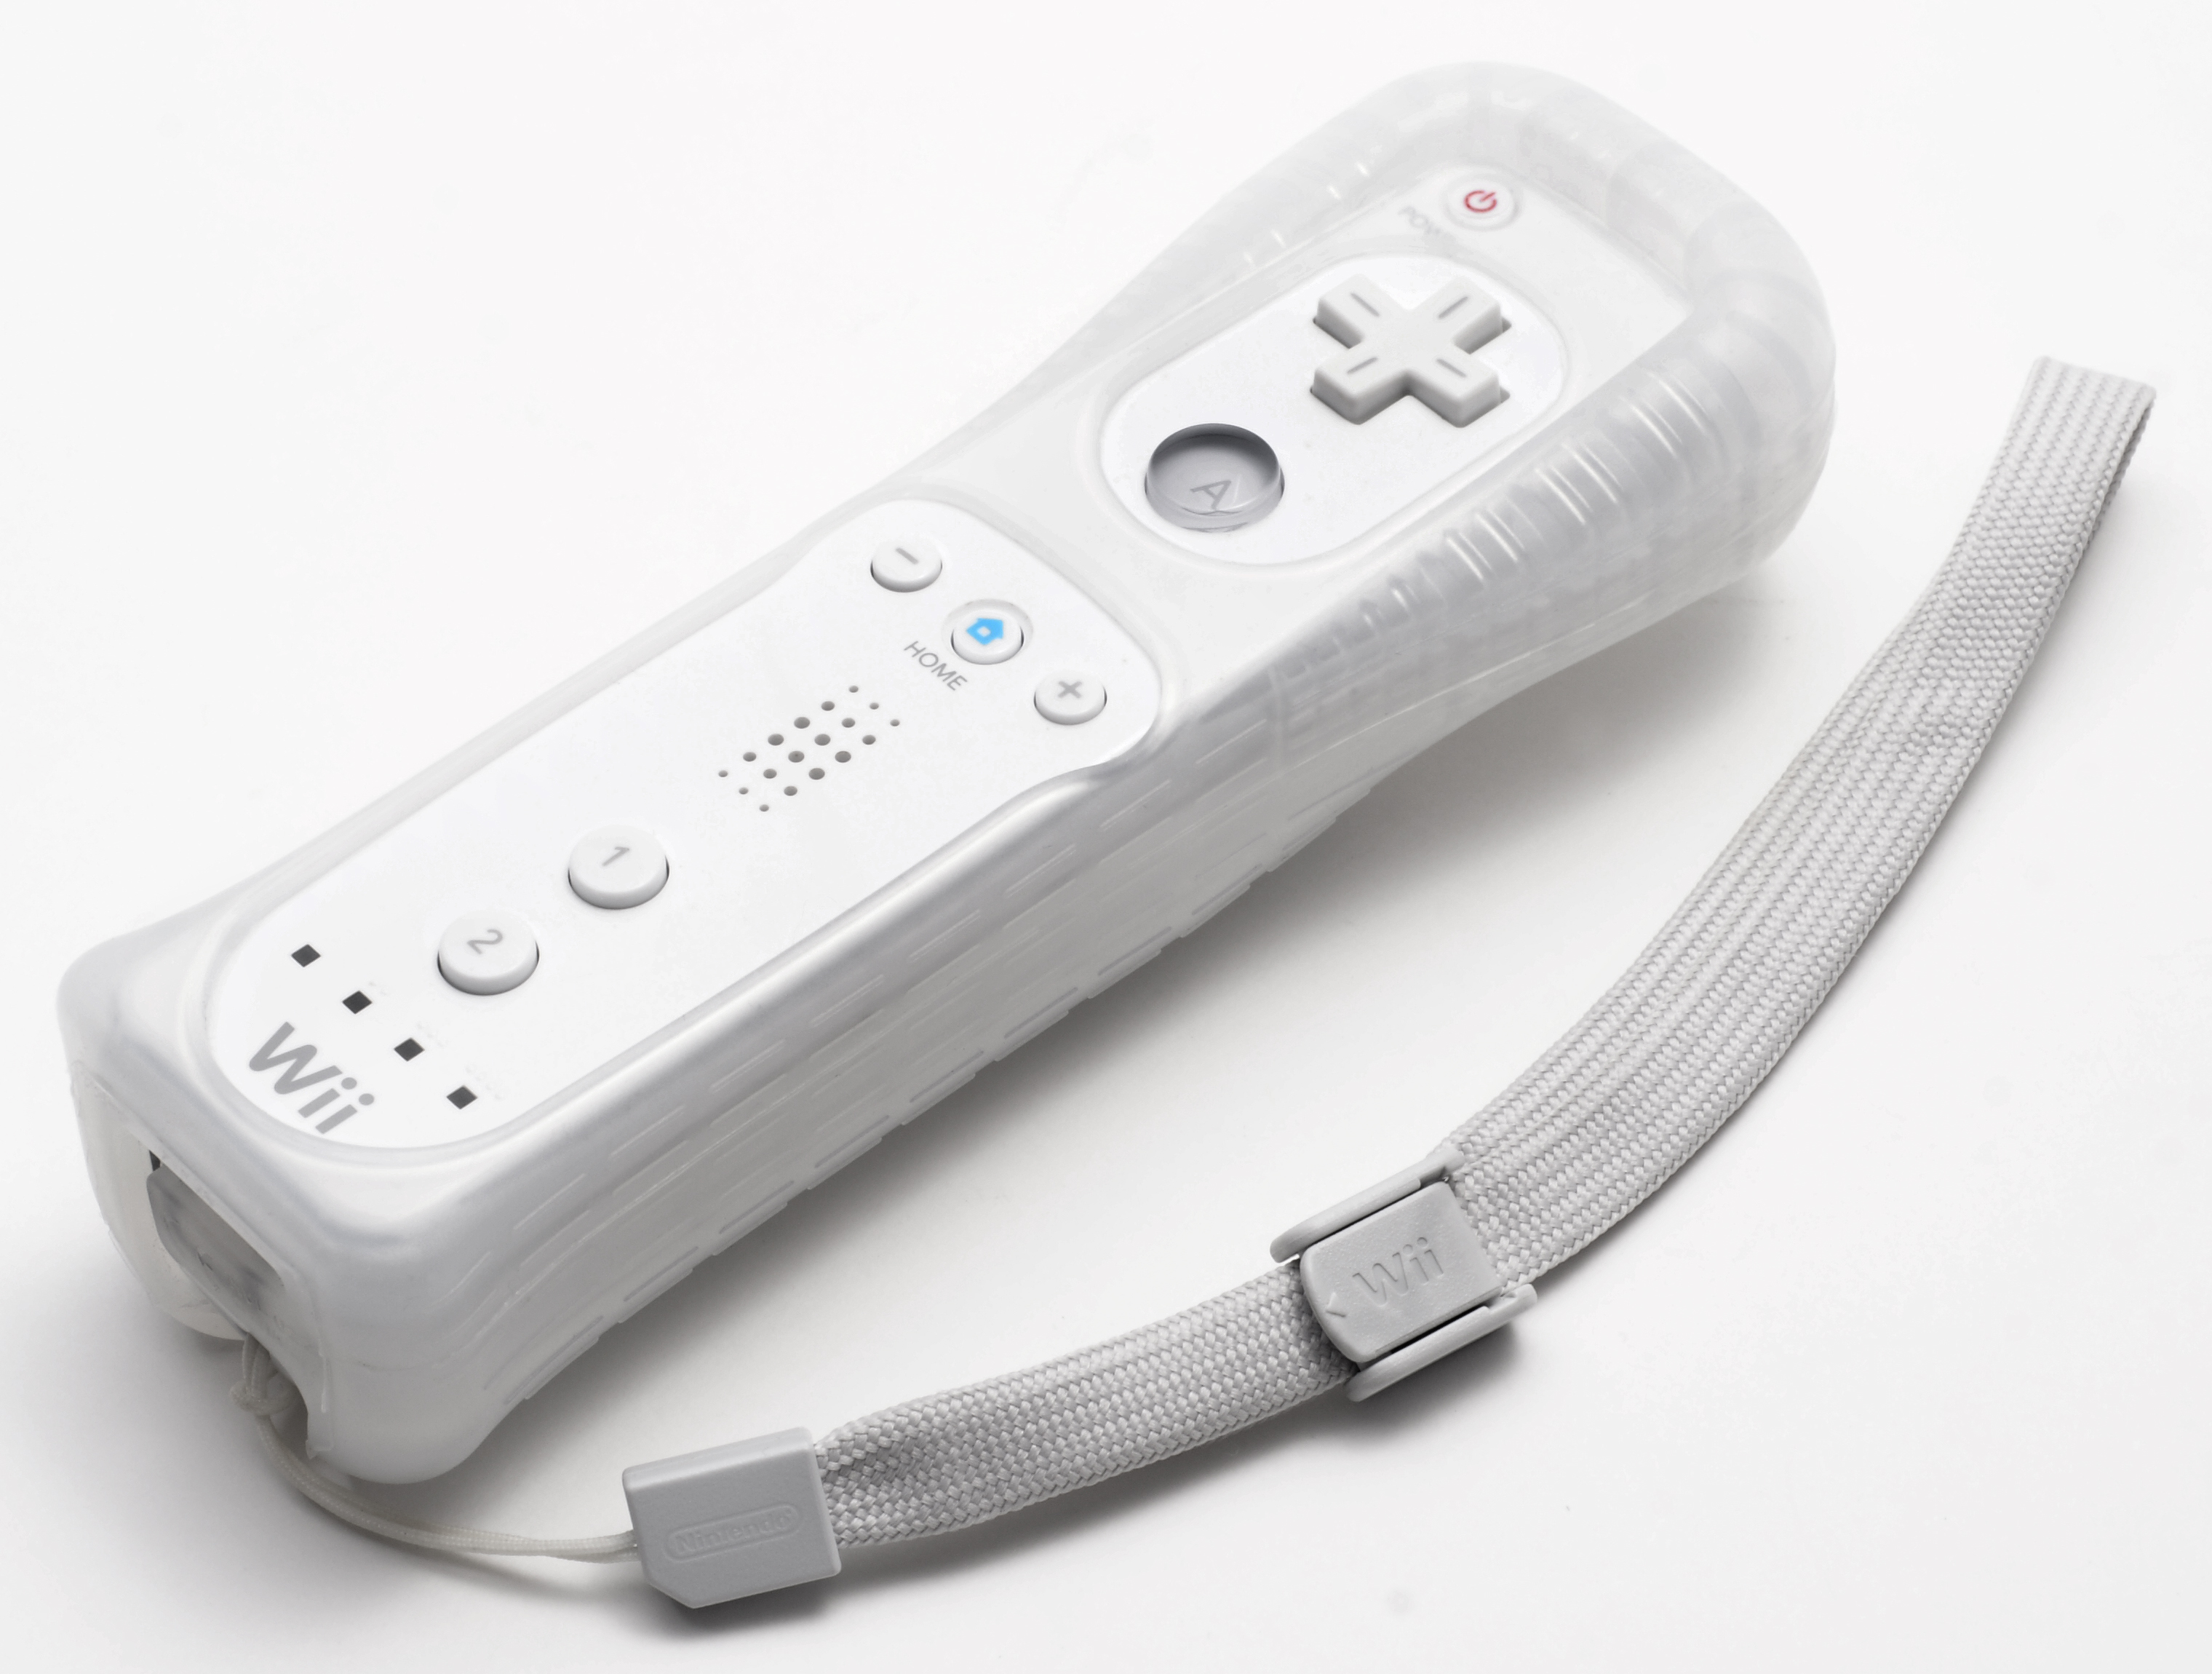
\includegraphics[width=0.4\textwidth]{images/intro/wii.jpg}
\end{figure}

